\section{Introducción}

El Problema del Vendedor Viajero (Traveling Salesman Problem, TSP) es un caso clásico de optimización combinatoria que busca encontrar la ruta más corta que permite visitar un conjunto de \( N \) ciudades exactamente una vez y regresar al punto de origen.
A pesar de su formulación simple, el TSP es un problema \textit{NP-hard}, por lo que no existe un algoritmo eficiente capaz de resolverlo de forma exacta en tiempo polinómico para todas las instancias. 

Este problema tiene gran relevancia práctica en ámbitos como la logística, la planificación de rutas, la manufactura o la biología computacional. Actualmente, técnicas heurísticas y metaheurísticas como lo son los algoritmos genéticos (GA) se han consolidado como herramientas efectivas para obtener soluciones aproximadas en tiempos razonables, especialmente en escenarios con gran número de ciudades o restricciones complejas.

En este trabajo se utiliza un algoritmo genético para resolver el TSP, aplicando operadores clásicos de cruce y mutación diseñados para preservar la validez de las permutaciones considerando que existen restricciones en las rutas. Entre los operadores de cruce se emplean:
\begin{itemize}\label{intro pmx/pbx}
    \item \textbf{PMX (Partially Mapped Crossover)}: mantiene la correspondencia entre segmentos de los padres mediante un mapeo parcial que evita duplicaciones.
    \item \textbf{PBX (Position-Based Crossover)}: conserva ciertas posiciones fijas del primer padre y completa el resto con el orden relativo del segundo.
\end{itemize}

Para la mutación se implementan:
\begin{itemize}
    \item \textbf{Scramble Mutation}: reordena aleatoriamente un subconjunto de ciudades, modificando el orden local sin alterar la estructura global.
    \item \textbf{Block Transpose Mutation}: intercambia bloques completos dentro de la ruta, explorando nuevas configuraciones manteniendo la coherencia de cada bloque.
\end{itemize}

Las distancias entre ciudades se calcularon mediante la fórmula del \textit{haversine}, que toma en cuenta la curvatura terrestre para obtener una medida más realista entre coordenadas geográficas.

Finalmente, al extender el TSP hacia versiones con \textbf{restricciones en las rutas}, se deben considerar factores adicionales como:
\begin{itemize}
    \item \textbf{Rutas prohibidas o tabúes}: pares de ciudades que no pueden conectarse directamente.
    \item \textbf{Penalizaciones adaptativas}: mecanismos que ajustan la función de aptitud para desalentar soluciones que violen restricciones.
\end{itemize}

La incorporación de estas restricciones transforma el ejercicio del TSP clásico en una variante más acercada a la realidad, representando escenarios reales para la distribución de mercancías o la planificación de rutas bajo limitaciones operativas.

\subsection{Ciudades}\label{lista_ciudades}
Para este ejercicio se utilizaron las siguientes ciudades europeas junto con su etiqueta correspondiente:
\begin{multicols}{3}
    \begin{itemize}
        \item 1 --- Berlin
        \item 2 --- Hamburg
        \item 3 --- Stutgart
        \item 4 --- Munich
        \item 5 --- Paris
        \item 6 --- Lyon
        \item 7 --- Bordeaux
        \item 8 --- Toulouse
        \item 9 --- Amsterdam
        \item 10 ---Brussels
        \item 11 ---Luxembourg
        \item 12 ---Zurich
        \item 13 ---Geneva
        \item 14 ---Vienna
        \item 15 ---Linz
        \item 16 ---Roma
        \item 17 ---Florencia
        \item 18 ---Napoles
    \end{itemize}
\end{multicols}

\begin{figure}[H]
    \centering
    
\includegraphics[width=0.75\textwidth]{rsc/img/intro/ciudades.png}
    \caption{Ciudades consideradas en el TSP.}\label{fig:ciudades}
\end{figure}

\subsection{Cálculo de Distancias (Matriz de Haversine)}\label{calculo_distancias}

Para calcular las distancias entre las ciudades, se utilizó la fórmula de haversine, que permite determinar la distancia entre dos puntos 
en la superficie de una esfera a partir de sus coordenadas de latitud y longitud. Esta fórmula es especialmente útil para 
distancias geográficas, ya que considera la curvatura de la Tierra.

\begin{figure}[H]
    \centering
    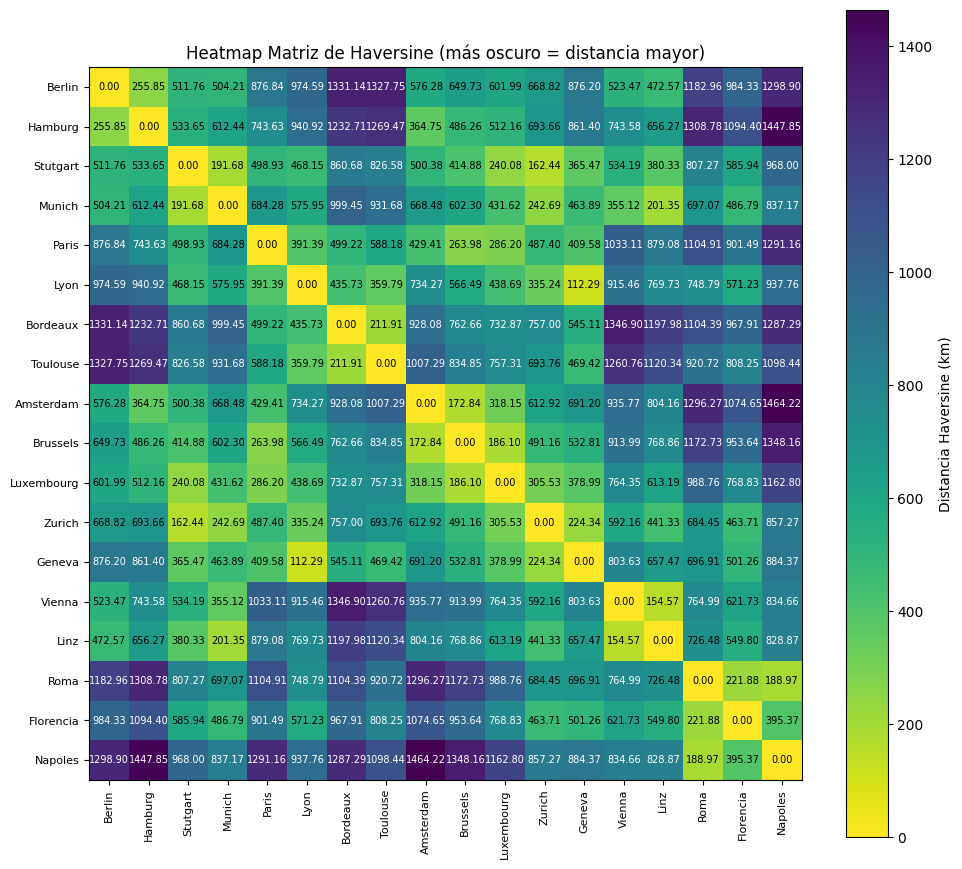
\includegraphics[width=0.85\textwidth]{rsc/img/intro/matriz_distancias.png}
    \caption{Matriz de distancias entre las ciudades consideradas en el TSP.}\label{fig:matriz_haversine}
\end{figure}

Como se puede ver en la figura~\ref{fig:matriz_haversine}, la matriz muestra las distancias en kilómetros entre cada par de ciudades,
en un heatmap donde los colores más oscuros representan distancias mayores y los colores más claros distancias menores. 
Esto nos proporciona una visión clara de las relaciones espaciales entre las ciudades, lo cual es fundamental para la optimización del TSP.\@